\documentclass[handout]{ximera}

\input{../preamble}


\title{Matrices as Transformations}
\author{Brad Findell}

\begin{document}
\begin{abstract}
Exercises about matrices as transformations.  
\end{abstract}
\maketitle

\begin{question}
The following figures show transformations that have mapped the unit square formed by the standard basis vectors to the other quadrilateral shown in the figure.  Which of the figures show a transformation that could be accomplished by the mapping 
\[
\begin{bmatrix} x' \\ y' \end{bmatrix} = A \begin{bmatrix} x \\ y \end{bmatrix} 
\]
for some $2\times2$ matrix $A$? 
\begin{multipleChoice}
\choice{ 
  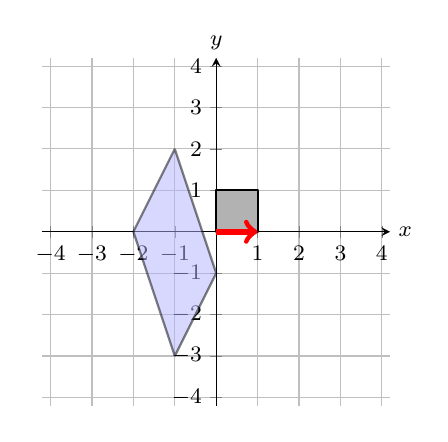
\begin{tikzpicture}
      \begin{axis}%
        [
	  xmin=-4.2,xmax=4.2,
          ymin=-4.2,ymax=4.2,
          xlabel=$x$,ylabel=$y$,
          axis lines=center,
          every axis y label/.style={at=(current axis.above origin),anchor=south},
          every axis x label/.style={at=(current axis.right of origin),anchor=west},
          clip=false,
	  grid =major,
          width=6cm,
          height=6cm,
          xtick={-4,-3,...,4},
          ytick={-4,-3,...,4},
	]
	\footnotesize
        \addplot[line join =bevel,black, thick,fill=black!30!white] coordinates{
          (0,0) (0,1) (1,1) (1,0) (0,0) (0,1)
          };
        \addplot [->,line width=2pt,color=red] coordinates{(0.,0.)  (1.,0.)};
        \addplot[line join =bevel,black, thick,fill=blue!30!white,opacity=0.5] coordinates{
		(0,-1) (-1,-3) (-2,0) (-1,2) (0,-1)
	};
        %\draw [->,line width=0.8pt,color=red] (0.,0.) -- (1.,0.);
      \end{axis}
    \end{tikzpicture}
    }
\choice{
  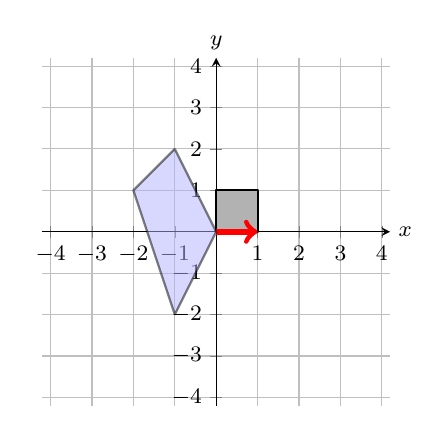
\begin{tikzpicture}
      \begin{axis}%
        [
	  xmin=-4.2,xmax=4.2,
          ymin=-4.2,ymax=4.2,
          xlabel=$x$,ylabel=$y$,
          axis lines=center,
          every axis y label/.style={at=(current axis.above origin),anchor=south},
          every axis x label/.style={at=(current axis.right of origin),anchor=west},
          clip=false,
	  grid =major,
          width=6cm,
          height=6cm,
          xtick={-4,-3,...,4},
          ytick={-4,-3,...,4},
	]
	\footnotesize
        \addplot[line join =bevel,black, thick,fill=black!30!white] coordinates{
          (0,0) (0,1) (1,1) (1,0) (0,0) (0,1)
          };
        \addplot [->,line width=2pt,color=red] coordinates{(0.,0.)  (1.,0.)};
        \addplot[line join =bevel,black, thick,fill=blue!30!white,opacity=0.5] coordinates{
		(0,0) (-1,-2) (-2,1) (-1,2) (0,0)
	};
        %\draw [->,line width=0.8pt,color=red] (0.,0.) -- (1.,0.);
      \end{axis}
    \end{tikzpicture}
    }
  \choice[correct]{ 
  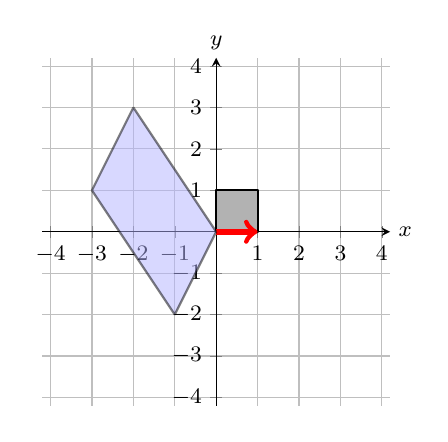
\begin{tikzpicture}
      \begin{axis}%
        [
	  xmin=-4.2,xmax=4.2,
          ymin=-4.2,ymax=4.2,
          xlabel=$x$,ylabel=$y$,
          axis lines=center,
          every axis y label/.style={at=(current axis.above origin),anchor=south},
          every axis x label/.style={at=(current axis.right of origin),anchor=west},
          clip=false,
	  grid =major,
          width=6cm,
          height=6cm,
          xtick={-4,-3,...,4},
          ytick={-4,-3,...,4},
	]
	\footnotesize
        \addplot[line join =bevel,black, thick,fill=black!30!white] coordinates{
          (0,0) (0,1) (1,1) (1,0) (0,0) (0,1)
          };
        \addplot [->,line width=2pt,color=red] coordinates{(0.,0.)  (1.,0.)};
        \addplot[line join =bevel,black, thick,fill=blue!30!white,opacity=0.5] coordinates{
		(0,0) (-1,-2) (-3,1) (-2,3) (0,0)
	};
        %\draw [->,line width=0.8pt,color=red] (0.,0.) -- (1.,0.);
      \end{axis}
    \end{tikzpicture}
    }
\end{multipleChoice}
\begin{question}
Correct!  Reasons for my choice:

Consider the vertices of the unit square:  
\begin{enumerate}
\item First vertex: The origin must be mapped to the $\answer[format=string]{origin}$.  
\item Second and third vertex: The images $Ae_1$ and $Ae_2$ must be vectors from the origin. 
\item Fourth vertex:  By linearity, $A(e_1+e_2) = Ae_1+Ae_2$, which means that the four vertex must be the vector sum of the first two.  By the $\answer[format=string]{parallelogram}$ rule, the vector sum $Ae_1+Ae_2$ is the diagonal of the $\answer[format=string]{parallelogram}$ formed by $Ae_1$ and $Ae_2$.  
\end{enumerate}
\begin{question}
Assuming the red arrow is mapped to the second quadrant, what is the matrix $A$? 
\[
A = \begin{bmatrix} \answer{-2} & \answer{-1} \\ \answer{3} & \answer{-2} \end{bmatrix}
\]
\end{question}
\end{question}
\end{question}
\end{document}
